\section{Usability Guidelines}\label{Usability Guidelines}

%\subsection{Offer informative feedback}
%-

%\subsection{Match between system and the real world}
%-
%\subsection{Grant the user control and freedom}
%-
\subsection{Consistency and standards}\label{consistency}
Rend 'n Lend provides an external consistency. \\
The searchbar is at the top in the middle of the page and the user profile is on the top right hand corner. The logo is on the top left hand corner. This arrangement can also be observed on many other websites, especially online stores. 

	\begin{figure}[H]
		\centering
		
\includegraphics[width=\linewidth]{abb/1_usability_guidelines/heuristic_constiency.png}
		\caption{consistency heuristic}
		\label{fig:heuristic_constiency}
	\end{figure}

\subsection{Support the user in avoiding errors}
When a rental transaction takes place, all agreed details must be recorded on a form. This form is prepared by the lender and must be approved by the renter. This way both parties can check all important information at a glance and misunderstandings or mistakes on both sides can be prevented. \\
	By listing the prices, the renter will not be surprised by any hidden costs.\\
		\begin{figure}[H]
		\centering
		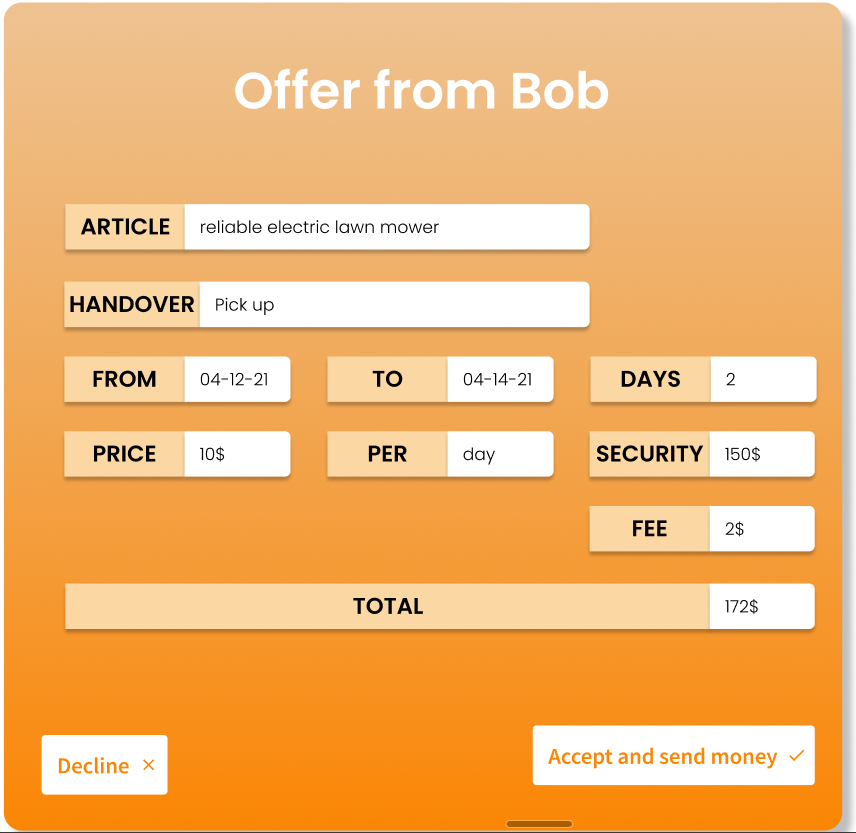
\includegraphics[width=0.7\linewidth]{abb/1_usability_guidelines/heuristic_avoid_errors.png}
		\caption{avoiding errors heuristic}
		\label{fig:heuristic_avoiding_errors}
	\end{figure}

\subsection{Minimize mental stress}
The user should be taken by the hand and guided through the entire process. The pages are kept simple and the icons are large and easy to understand. Advertising is discreetly integrated, but care is taken to ensure that it is clearly marked so that the user does not accidentally click on it. \\
All this ensures that stress and frustration are kept to a minimum.

%\subsection{Enable flexible and efficient use}
%-
%\subsection{Simple and aesthetic design}
%-
%\subsection{Allow for easy troubleshooting}
%-
%\subsection{Offer help and documentation}
%-


%\subsection{Aesthetic-Usability Effect}
%-
\subsection{Jakob's Law}
As described in section \ref{consistency}, the header is arranged exactly as it is on many other pages. This allows the user to quickly find his way around.

%\subsection{Von Restorff Effect}
%evtl die werbung ?
\subsection{Law of common region}
	\begin{wrapfigure}{l}{0.3\linewidth}
	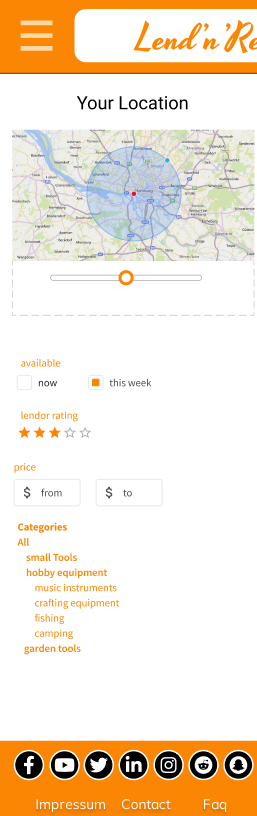
\includegraphics[width=0.3\textwidth]{abb/1_usability_guidelines/heuristic_region.png}
	\caption{Common region heuristic}
	\label{fig:heuristic_common_region}
\end{wrapfigure}
Multiple objects are displayed in a delimited region. \\
This heuristic can be observed well in the fold-out menu on the left side. In figure \ref{fig:heuristic_common_region}, for example, details of the search can be specified.



%\subsection{Fitts's Law}
%-
%\subsection{Law of Proximity}
%-
%\subsection{Pareto Principle}
%-
\subsection{Law of similarity}
Care is taken to ensure that sections are always presented in a uniform manner. On the search page, figure \ref{fig:search}, you can easily see that the articles are all of the same size and are displayed according to the same scheme.\\
 Also on the home page the categories follow a similar scheme, see figure \ref{fig:8start}. The buttons are also consistent.
%\subsection{Occam's Razor}
%-
\subsection{Law of uniform connectedness}

\definecolor{lender}{HTML}{84d7fb}
\definecolor{renter}{HTML}{fb8604}

From the beginning, the page separates by color according to the role of the user. If the user is a \textcolor{lender}{lender} , which means he has at least one item on offer, a light blue color is used. \\ If the user only borrows things, he is a \textcolor{renter}{renter} and an orange color is used. This can be seen very well on the landing page, figure \ref{fig:1landing}.

